\documentclass{standalone}
\usepackage{tikz}
\usetikzlibrary{patterns, positioning}

\begin{document}
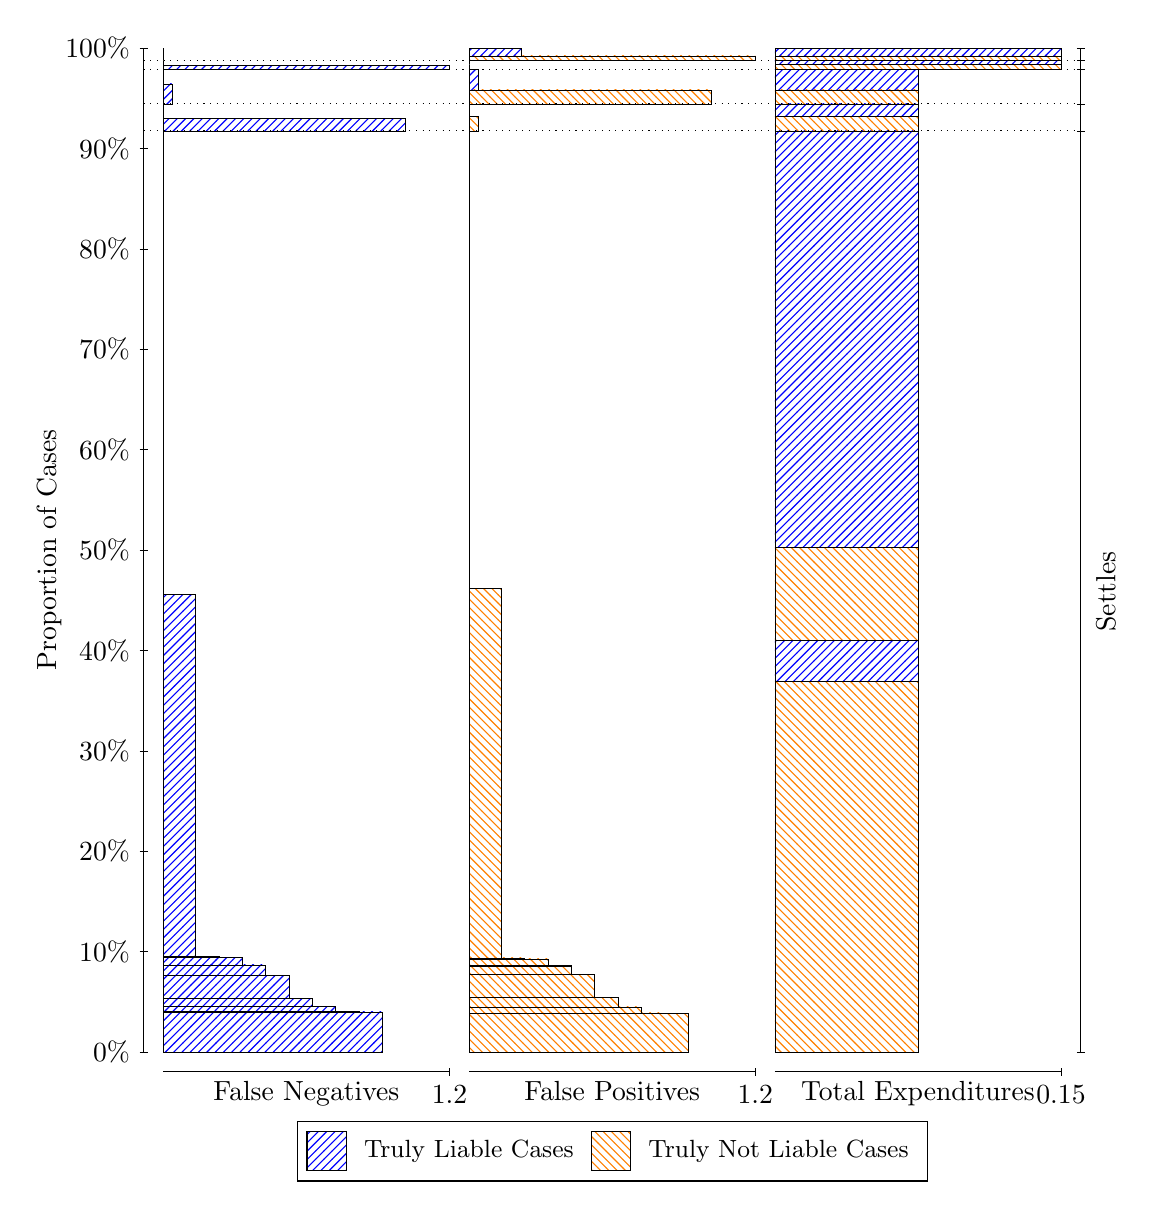
\begin{tikzpicture}
\draw[black, very thin] (1.5,1.75) -- (1.5,14.5);
\node[rotate=90, anchor=center] at (0.3, 8.125) {Proportion of Cases};
\draw[black, very thin] (1.45,1.75) -- (1.55,1.75);
\node[anchor=east] at (1.45, 1.75) {0\%};
\draw[black, very thin] (1.45,3.025) -- (1.55,3.025);
\node[anchor=east] at (1.45, 3.025) {10\%};
\draw[black, very thin] (1.45,4.3) -- (1.55,4.3);
\node[anchor=east] at (1.45, 4.3) {20\%};
\draw[black, very thin] (1.45,5.575) -- (1.55,5.575);
\node[anchor=east] at (1.45, 5.575) {30\%};
\draw[black, very thin] (1.45,6.85) -- (1.55,6.85);
\node[anchor=east] at (1.45, 6.85) {40\%};
\draw[black, very thin] (1.45,8.125) -- (1.55,8.125);
\node[anchor=east] at (1.45, 8.125) {50\%};
\draw[black, very thin] (1.45,9.4) -- (1.55,9.4);
\node[anchor=east] at (1.45, 9.4) {60\%};
\draw[black, very thin] (1.45,10.675) -- (1.55,10.675);
\node[anchor=east] at (1.45, 10.675) {70\%};
\draw[black, very thin] (1.45,11.95) -- (1.55,11.95);
\node[anchor=east] at (1.45, 11.95) {80\%};
\draw[black, very thin] (1.45,13.225) -- (1.55,13.225);
\node[anchor=east] at (1.45, 13.225) {90\%};
\draw[black, very thin] (1.45,14.5) -- (1.55,14.5);
\node[anchor=east] at (1.45, 14.5) {100\%};

\draw[black, very thin] (13.4,1.75) -- (13.4,14.5);
\draw[black, very thin] (13.35,1.75) -- (13.45,1.75);
\node[anchor=west] at (13.35, 1.75) {};
\draw[black, very thin] (13.35,13.448) -- (13.45,13.448);
\node[anchor=west] at (13.35, 13.448) {};
\draw[black, very thin] (13.35,13.79) -- (13.45,13.79);
\node[anchor=west] at (13.35, 13.79) {};
\draw[black, very thin] (13.35,14.224) -- (13.45,14.224);
\node[anchor=west] at (13.35, 14.224) {};
\draw[black, very thin] (13.35,14.341) -- (13.45,14.341);
\node[anchor=west] at (13.35, 14.341) {};
\draw[black, very thin] (13.35,14.5) -- (13.45,14.5);
\node[anchor=west] at (13.35, 14.5) {};

\draw[black, very thin, pattern color=blue, pattern=north east lines] (1.75,1.75) rectangle (4.5306,2.2597);
\draw[black, very thin, pattern color=blue, pattern=north east lines] (1.75,2.2597) rectangle (4.234,2.2668);
\draw[black, very thin, pattern color=blue, pattern=north east lines] (1.75,2.2668) rectangle (3.9374,2.3268);
\draw[black, very thin, pattern color=blue, pattern=north east lines] (1.75,2.3268) rectangle (3.6408,2.4346);
\draw[black, very thin, pattern color=blue, pattern=north east lines] (1.75,2.4346) rectangle (3.3442,2.7245);
\draw[black, very thin, pattern color=blue, pattern=north east lines] (1.75,2.7245) rectangle (3.0476,2.8562);
\draw[black, very thin, pattern color=blue, pattern=north east lines] (1.75,2.8562) rectangle (2.751,2.9493);
\draw[black, very thin, pattern color=blue, pattern=north east lines] (1.75,2.9493) rectangle (2.4544,2.9658);
\draw[black, very thin, pattern color=blue, pattern=north east lines] (1.75,2.9658) rectangle (2.1578,7.5575);
\draw[black, very thin, pattern color=orange, pattern=north west lines] (1.75,7.5575) rectangle (1.75,13.448);
\draw[black, very thin, pattern color=blue, pattern=north east lines] (1.75,13.448) rectangle (4.8272,13.609);
\draw[black, very thin, pattern color=orange, pattern=north west lines] (1.75,13.609) rectangle (1.75,13.79);
\draw[black, very thin, pattern color=blue, pattern=north east lines] (1.75,13.79) rectangle (1.8612,14.044);
\draw[black, very thin, pattern color=orange, pattern=north west lines] (1.75,14.044) rectangle (1.75,14.224);
\draw[black, very thin, pattern color=blue, pattern=north east lines] (1.75,14.224) rectangle (5.3833,14.275);
\draw[black, very thin, pattern color=orange, pattern=north west lines] (1.75,14.275) rectangle (1.75,14.341);
\draw[black, very thin, pattern color=orange, pattern=north west lines] (1.75,14.341) rectangle (1.75,14.399);
\draw[black, very thin, pattern color=blue, pattern=north east lines] (1.75,14.399) rectangle (1.75,14.5);
\draw[black, very thin, pattern color=orange, pattern=north west lines] (5.6333,1.75) rectangle (8.4139,2.2392);
\draw[black, very thin, pattern color=orange, pattern=north west lines] (5.6333,2.2392) rectangle (8.1173,2.247);
\draw[black, very thin, pattern color=orange, pattern=north west lines] (5.6333,2.247) rectangle (7.8207,2.3232);
\draw[black, very thin, pattern color=orange, pattern=north west lines] (5.6333,2.3232) rectangle (7.5241,2.4476);
\draw[black, very thin, pattern color=orange, pattern=north west lines] (5.6333,2.4476) rectangle (7.2276,2.7372);
\draw[black, very thin, pattern color=orange, pattern=north west lines] (5.6333,2.7372) rectangle (6.931,2.837);
\draw[black, very thin, pattern color=orange, pattern=north west lines] (5.6333,2.837) rectangle (6.931,2.8536);
\draw[black, very thin, pattern color=orange, pattern=north west lines] (5.6333,2.8536) rectangle (6.6344,2.9313);
\draw[black, very thin, pattern color=orange, pattern=north west lines] (5.6333,2.9313) rectangle (6.3378,2.9461);
\draw[black, very thin, pattern color=orange, pattern=north west lines] (5.6333,2.9461) rectangle (6.0412,7.6408);
\draw[black, very thin, pattern color=blue, pattern=north east lines] (5.6333,7.6408) rectangle (5.6333,13.448);
\draw[black, very thin, pattern color=orange, pattern=north west lines] (5.6333,13.448) rectangle (5.7446,13.629);
\draw[black, very thin, pattern color=blue, pattern=north east lines] (5.6333,13.629) rectangle (5.6333,13.79);
\draw[black, very thin, pattern color=orange, pattern=north west lines] (5.6333,13.79) rectangle (8.7105,13.969);
\draw[black, very thin, pattern color=blue, pattern=north east lines] (5.6333,13.969) rectangle (5.7446,14.224);
\draw[black, very thin, pattern color=orange, pattern=north west lines] (5.6333,14.224) rectangle (5.6333,14.29);
\draw[black, very thin, pattern color=blue, pattern=north east lines] (5.6333,14.29) rectangle (5.6333,14.341);
\draw[black, very thin, pattern color=orange, pattern=north west lines] (5.6333,14.341) rectangle (9.2667,14.399);
\draw[black, very thin, pattern color=blue, pattern=north east lines] (5.6333,14.399) rectangle (6.3007,14.5);
\draw[black, very thin, pattern color=orange, pattern=north west lines] (9.5167,1.75) rectangle (11.333,6.4595);
\draw[black, very thin, pattern color=blue, pattern=north east lines] (9.5167,6.4595) rectangle (11.333,6.9763);
\draw[black, very thin, pattern color=orange, pattern=north west lines] (9.5167,6.9763) rectangle (11.333,8.1576);
\draw[black, very thin, pattern color=blue, pattern=north east lines] (9.5167,8.1576) rectangle (11.333,13.448);
\draw[black, very thin, pattern color=orange, pattern=north west lines] (9.5167,13.448) rectangle (11.333,13.629);
\draw[black, very thin, pattern color=blue, pattern=north east lines] (9.5167,13.629) rectangle (11.333,13.79);
\draw[black, very thin, pattern color=orange, pattern=north west lines] (9.5167,13.79) rectangle (11.333,13.969);
\draw[black, very thin, pattern color=blue, pattern=north east lines] (9.5167,13.969) rectangle (11.333,14.224);
\draw[black, very thin, pattern color=orange, pattern=north west lines] (9.5167,14.224) rectangle (13.15,14.29);
\draw[black, very thin, pattern color=blue, pattern=north east lines] (9.5167,14.29) rectangle (13.15,14.341);
\draw[black, very thin, pattern color=orange, pattern=north west lines] (9.5167,14.341) rectangle (13.15,14.399);
\draw[black, very thin, pattern color=blue, pattern=north east lines] (9.5167,14.399) rectangle (13.15,14.5);
\draw[black, dotted] (1.5,13.448) -- (13.4,13.448);
\draw[black, dotted] (1.5,13.79) -- (13.4,13.79);
\draw[black, dotted] (1.5,14.224) -- (13.4,14.224);
\draw[black, dotted] (1.5,14.341) -- (13.4,14.341);
\draw[black, very thin] (1.75,1.5) -- (5.3833,1.5);
\node[anchor=north] at (3.5667, 1.5) {False Negatives};
\draw[black, very thin] (5.3833,1.45) -- (5.3833,1.55);
\node[anchor=north] at (5.3833, 1.45) {1.2};

\draw[black, very thin] (5.6333,1.5) -- (9.2667,1.5);
\node[anchor=north] at (7.45, 1.5) {False Positives};
\draw[black, very thin] (9.2667,1.45) -- (9.2667,1.55);
\node[anchor=north] at (9.2667, 1.45) {1.2};

\draw[black, very thin] (9.5167,1.5) -- (13.15,1.5);
\node[anchor=north] at (11.333, 1.5) {Total Expenditures};
\draw[black, very thin] (13.15,1.45) -- (13.15,1.55);
\node[anchor=north] at (13.15, 1.45) {0.15};

\node[black, centered, rotate=90] at (13.72, 7.5991) {Settles};





\draw (7.449999999999999,1.5) node[draw=none] (baseCoordinate) {};
\begin{scope}[align=center]
        \matrix[scale=0.5, draw=black, below=0.5cm of baseCoordinate, nodes={draw}, column sep=0.1cm]{
            \node[rectangle, draw, minimum width=0.5cm, minimum height=0.5cm, pattern=north east lines, pattern color=blue] {}; &
            \node[draw=none, font=\small] (B) {Truly Liable Cases}; &
            \node[rectangle, draw, minimum width=0.5cm, minimum height=0.5cm, pattern=north west lines, pattern color=orange] {}; &
            \node[draw=none, font=\small] (B) {Truly Not Liable Cases}; \\
            };
\end{scope}

\end{tikzpicture}
\end{document}